\documentclass[]{article}
\usepackage{lmodern}
\usepackage{amssymb,amsmath}
\usepackage{ifxetex,ifluatex}
\usepackage{fixltx2e} % provides \textsubscript
\ifnum 0\ifxetex 1\fi\ifluatex 1\fi=0 % if pdftex
  \usepackage[T1]{fontenc}
  \usepackage[utf8]{inputenc}
\else % if luatex or xelatex
  \ifxetex
    \usepackage{mathspec}
  \else
    \usepackage{fontspec}
  \fi
  \defaultfontfeatures{Ligatures=TeX,Scale=MatchLowercase}
  \newcommand{\euro}{€}
\fi
% use upquote if available, for straight quotes in verbatim environments
\IfFileExists{upquote.sty}{\usepackage{upquote}}{}
% use microtype if available
\IfFileExists{microtype.sty}{%
\usepackage{microtype}
\UseMicrotypeSet[protrusion]{basicmath} % disable protrusion for tt fonts
}{}
\usepackage[margin=1in]{geometry}
\usepackage{hyperref}
\PassOptionsToPackage{usenames,dvipsnames}{color} % color is loaded by hyperref
\hypersetup{unicode=true,
            pdfborder={0 0 0},
            breaklinks=true}
\urlstyle{same}  % don't use monospace font for urls
\usepackage{longtable,booktabs}
\usepackage{graphicx,grffile}
\makeatletter
\def\maxwidth{\ifdim\Gin@nat@width>\linewidth\linewidth\else\Gin@nat@width\fi}
\def\maxheight{\ifdim\Gin@nat@height>\textheight\textheight\else\Gin@nat@height\fi}
\makeatother
% Scale images if necessary, so that they will not overflow the page
% margins by default, and it is still possible to overwrite the defaults
% using explicit options in \includegraphics[width, height, ...]{}
\setkeys{Gin}{width=\maxwidth,height=\maxheight,keepaspectratio}
\setlength{\parindent}{0pt}
\setlength{\parskip}{6pt plus 2pt minus 1pt}
\setlength{\emergencystretch}{3em}  % prevent overfull lines
\providecommand{\tightlist}{%
  \setlength{\itemsep}{0pt}\setlength{\parskip}{0pt}}
\setcounter{secnumdepth}{0}

%%% Use protect on footnotes to avoid problems with footnotes in titles
\let\rmarkdownfootnote\footnote%
\def\footnote{\protect\rmarkdownfootnote}

%%% Change title format to be more compact
\usepackage{titling}

% Create subtitle command for use in maketitle
\newcommand{\subtitle}[1]{
  \posttitle{
    \begin{center}\large#1\end{center}
    }
}

\setlength{\droptitle}{-2em}
  \title{}
  \pretitle{\vspace{\droptitle}}
  \posttitle{}
  \author{}
  \preauthor{}\postauthor{}
  \date{}
  \predate{}\postdate{}


\usepackage{graphicx,latexsym}
\usepackage{amssymb,amsthm,amsmath}
\usepackage{longtable,booktabs,setspace, dsfont, array}

% Redefines (sub)paragraphs to behave more like sections
\ifx\paragraph\undefined\else
\let\oldparagraph\paragraph
\renewcommand{\paragraph}[1]{\oldparagraph{#1}\mbox{}}
\fi
\ifx\subparagraph\undefined\else
\let\oldsubparagraph\subparagraph
\renewcommand{\subparagraph}[1]{\oldsubparagraph{#1}\mbox{}}
\fi

\begin{document}

\section{Modeling Rides and Riders}\label{model-chapter}

Complex statistical models can accurately model intricate processes. But
they also run the risk of overfitting to the data. To avoid this, we
build up our models from simple to complex, comparing the models with
cross validation to make sure the complexities introduced add real
value.

In this chapter we focus on building models that incorporate information
about rider, weather conditions, time of day, and ride length. In brief,
our models start with a logistic regression model considering only
ride-level variables, and formulate more complex models by adding
various terms. \autoref{tab:models} describes each model briefly along
with the models label.

\begin{longtable}[]{@{}ll@{}}
\caption{Brief descriptions of Models 1--6
\label{tab:models}}\tabularnewline
\toprule
\begin{minipage}[b]{0.13\columnwidth}\raggedright\strut
\textbf{Model}
\strut\end{minipage} &
\begin{minipage}[b]{0.72\columnwidth}\raggedright\strut
\textbf{Description}
\strut\end{minipage}\tabularnewline
\midrule
\endfirsthead
\toprule
\begin{minipage}[b]{0.13\columnwidth}\raggedright\strut
\textbf{Model}
\strut\end{minipage} &
\begin{minipage}[b]{0.72\columnwidth}\raggedright\strut
\textbf{Description}
\strut\end{minipage}\tabularnewline
\midrule
\endhead
\begin{minipage}[t]{0.13\columnwidth}\raggedright\strut
Model 1
\strut\end{minipage} &
\begin{minipage}[t]{0.72\columnwidth}\raggedright\strut
(Baseline) logistic regression
\strut\end{minipage}\tabularnewline
\begin{minipage}[t]{0.13\columnwidth}\raggedright\strut
Model 2
\strut\end{minipage} &
\begin{minipage}[t]{0.72\columnwidth}\raggedright\strut
Add rider intercepts
\strut\end{minipage}\tabularnewline
\begin{minipage}[t]{0.13\columnwidth}\raggedright\strut
Model 3
\strut\end{minipage} &
\begin{minipage}[t]{0.72\columnwidth}\raggedright\strut
Add trigonometric terms for time of day
\strut\end{minipage}\tabularnewline
\begin{minipage}[t]{0.13\columnwidth}\raggedright\strut
Model 4
\strut\end{minipage} &
\begin{minipage}[t]{0.72\columnwidth}\raggedright\strut
Additive model with cubic cyclic spline for time of day
\strut\end{minipage}\tabularnewline
\begin{minipage}[t]{0.13\columnwidth}\raggedright\strut
Model 5
\strut\end{minipage} &
\begin{minipage}[t]{0.72\columnwidth}\raggedright\strut
Additive model with spline for ride length
\strut\end{minipage}\tabularnewline
\begin{minipage}[t]{0.13\columnwidth}\raggedright\strut
Model 6
\strut\end{minipage} &
\begin{minipage}[t]{0.72\columnwidth}\raggedright\strut
Remove random rider intercepts from Model 4
\strut\end{minipage}\tabularnewline
\bottomrule
\end{longtable}

\subsection{Six Models for Probability of a Negative Ride
Rating}\label{ride-models}

\textbf{Model 1}, which we will use as the baseline for comparing
further models, is a multiple logistic regression model. Then, our first
model will be,

\[ \mathbb{P} (Y_i=1) = \text{logit}^{-1} (\alpha + X_i \beta),\]

where \(\alpha \in \mathbb{R}\) and \(\beta \in \mathbb{R}^p\) are
parameters to be estimated. (\(X\) is the matrix of rider-level
predictors specified at the end of \autoref{data-notation}.)

\begin{figure}[tbh]
\centering
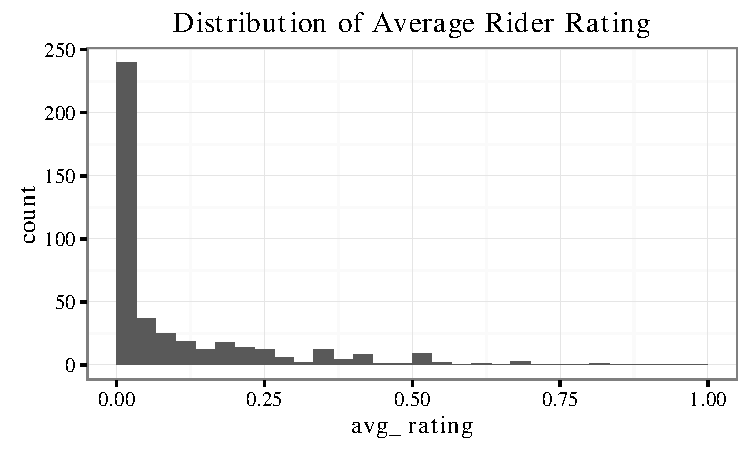
\includegraphics[angle = 0,scale = 1]{figure/rider_avgs.pdf}
\caption[The overall rates at which each rider gives a negative rating for a
ride varies greatly. This is our primary motivation for including rider intercepts
and predictors.]{\normalsize{The overall rates at which each rider gives a negative rating for a
ride varies greatly. This is our primary motivation for including rider intercepts
and predictors.}}
\label{fig:rider-avgs}
\end{figure}

Riders appear to have different tendencies to rate rides negatively more
often, as we note in \autoref{fig:rider-avgs}. In fact, many riders give
zero or nearly zero negative ratings. For \textbf{Model 2}, we account
for this variability by adding intercepts that vary by rider:

\begin{equation}
y_i \sim \text{Bernoulli} \left(
\text{logit}^{-1} \left( \alpha + \alpha_{j[i]} + X_i \beta \right)
\right),
\end{equation}

for \(i = 1, \ldots, n\).

Rider intercepts themselves aren't as interesting as how they deviate
from the mean, so we keep a fixed intercept \(\alpha\) and constrain the
rider intercepts, \(\alpha_j\), by specifying

\[\alpha_j \sim N(0, \sigma^2_\alpha).\]

Starting with \textbf{Model 3}, we address time of day,
\(t \in [0, 24)\) as a predictor. (We measure time of day in hours since
midnight.) We use time of day to account for the all daily trends that
may affect ratings, including as a simple way to model the overall
traffic level, which is difficult to model on its own. These patterns
are cyclic and very non-linear, so we can't time as a linear term. One
approach is to add sinusoidal terms with a period of one day. We would
be interested in fitting a term,

\[\beta \sin (T x^{\text{time}} + \phi).\]

Estimating \(\beta\) wouldn't be hard: we can easily estimate
coefficents of tranformed terms; it's more difficult to estimate \(T\)
and \(\phi\). But, we know that we want to restrict our terms to fitting
trends that happen over the course of one day, so we can set
\(T = 2 \pi / d\), where \(d\) is 24 hours or some fraction of that.

As for \(\phi\), a trignometric transformation reframes the estimation
of a phase shift parameter into the estimation of two coefficients for
trignometric functions with no phase shift:

\begin{align*}
\beta \sin (T x + \phi) &= 
\beta \left( \sin (T x) \cos (\phi) + \cos (T x) \sin (\phi) \right)\\
&= \beta \cos (\phi)) \sin (T x) + \sin (\phi) \cos (T x)\\
&= \beta_1 \sin (T x) + \beta_2 \cos (T x),
\end{align*}

where \(\beta_1 = \beta \cos (\phi)\) and \(\beta_2 = \sin (\phi).\) At
this point, we are now just estimating the coefficients of a couple of
transformed variables, which can easily be done in any package that does
generalized linear regressions.

We also want to take into account that weekday hourly patterns may be
different than weekend patterns. We use a variable \(X^\text{weekend}\)
that serves as a weekend indicator. For Model 3, we add two sets of
sinusoidal terms: one set for weekdays and one for weekends. More
explicitly, we define the model,

\begin{equation}
\begin{split}
\mathbb{P} (Y_i=1) = \text{logit}^{-1} (&\alpha + \alpha_{j[i]} + X_i \beta \\
&+ X^\text{weekend} \cdot [\beta^{t1} \sin(T \cdot t) + \beta^{t2} \cos (T \cdot t)\\
&+ \beta^{t3} \sin(T/2 \cdot t) + \beta^{t4} \cos (T/2 \cdot t)]\\
&+ (1 - X^\text{weekend}) \cdot [\beta^{t1} \sin(T \cdot t) + \beta^{t2} \cos (T \cdot t)\\
&+ \beta^{t3} \sin(T/2 \cdot t) + \beta^{t4} \cos (T/2 \cdot t))].
\end{split}
\end{equation}

For \textbf{Model 4} we abandon parametric methods and use a cyclic
non-parametric smoother to model time of day, making our model,

\begin{equation}
y_i \sim \text{Bernoulli} \left(
\text{logit}^{-1} \left( \alpha + \alpha_{j[i]} + X_i \beta + 
f^\text{time} (t_i)  \right)
\right),
\end{equation}

for \(i = 1, \ldots, n\), where \(\alpha_j\) is specified like Model 2
and \(f^\text{time}\) is a cyclic cubic spline term, with knots at 0, 3,
6, 9, 12, 15, 18, 21, and 24 (0, again) hours.

\textbf{Model 5} extends Model 4 by adding a cubic spline for
ride\_length:

\begin{equation}
y_i \sim \text{Bernoulli} \left(
\text{logit}^{-1} \left( \alpha + \alpha_{j[i]} + X_i \beta + 
f^\text{time} (t_i) + f^\text{length} (x^\text{log.length}_i)  \right)
\right),
\end{equation}

for \(i = 1, \ldots, n\), where \(f^\text{length}\) is a cubic spline
smoother.

Finally, \textbf{Model 6} is identical to Model 5, but without the rider
intercepts:

\begin{equation}
y_i \sim \text{Bernoulli} \left(
\text{logit}^{-1} \left( \alpha + X_i \beta + 
f^\text{time} (t_i)  \right)
\right),
\end{equation}

for \(i = 1, \ldots, n\), where \(f^\text{time}\) is a cyclic cubic
spline term, with the same knots as in Model 4.

\subsection{Model Evaluation}\label{model-evaluation}

\begin{table}[htb]
\centering
\caption{Fit summaries for Models 1--6.\label{tab:modelfits}}
\begin{tabular}{lm{4in}rrr}
\toprule
\textbf{Model} & \textbf{Separation Plot} & \textbf{$\log (\mathcal{L})$} & \textbf{AIC} &
\textbf{AUC}$_{\text{CV}}$\footnotemark\\
\midrule
Model 1 & 
\includegraphics{figure/model1-sep.pdf}
& -4,786 & 9,586 & 0.552\\
Model 2 & 
\includegraphics{figure/model2-sep.pdf}
& -3,971 & 7,957 & 0.797\\
Model 3 & 
\includegraphics{figure/model3-sep.pdf}
& -3,923 & 7,877 & 0.802\\
Model 4 & 
\includegraphics{figure/model4-sep.pdf}
& -3,930 & 7,870 & 0.802\\
Model 5 & 
\includegraphics{figure/model5-sep.pdf}
& -3,928 & 7,878 & 0.803\\
Model 6 & 
\includegraphics{figure/model6-sep.pdf}
& -4,713 & 9,455 & 0.601\\
\bottomrule
\end{tabular}
\end{table}

\footnotetext{Area under ROC curve estimated with  10-fold cross-validation.}

To fit the data, we got all of the rides in Portland, OR from December
3, 2014 to February 8, 2016 for riders that had over 20 rated rides.
There were 25,397 rides, 14,032 of which were rated. Overall, 10.88
percent of these rides were given a negative rating. There were 138
riders in the data set.

The separation plots in \autoref{tab:modelfits} give a clear initial
picture of how these model fits compare. Model 1 performs very poorly
compared to those that include rider intercepts, assigning the same
probability to most observations. Models that include the rider
intercept perform similarly to each other. The log likelihoods and AIC
scores, shown in \autoref{tab:modelfits}, corroborate this. Adding time
dependency doesn't seem to impact predictive ability. We will see later,
however, that it gives a fascinating result to interpret.

The gains from the rider intercepts are great, but we are compelled to
ask: how much of that gain could have been achieved with randomly chosen
groups? \textit{i.e.} if riders were randomly assigned to rides, would
the flexibility in the model created by allowing intercepts to vary
increase predictive performance to the same degree? To test this, we ran
a Model 4 after we randomly assign the rides a rider. This quick test
nullified this skepticism, as you can see in the resulting separation
plots in \autoref{fig:sep-plots-intercept-test}.

\begin{figure}[tbh]
\centering
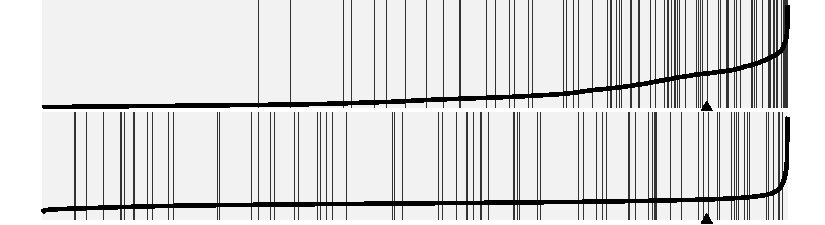
\includegraphics[angle = 0,scale = 1]{figure/intercept_test_plot.pdf}
\caption[Separation plots for models 2 compared to a similar model where
riders are randomly assigned to rides. This test demonstrates that the 
improvement in predictive performance provided by the rider intercepts
was not coincidence.]{\normalsize{Separation plots for models 2 compared to a similar model where
riders are randomly assigned to rides. This test demonstrates that the 
improvement in predictive performance provided by the rider intercepts
was not coincidence.}}
\label{fig:sep-plots-intercept-test}
\end{figure}

\subsection{Model Results}\label{model-results}

\begin{table}[htb]
\centering
\def\arraystretch{1.3}
\caption[Regression coefficients for Models 1, 2, 4, and 6.]{Regression coefficients for Model 1, Model 2, Model 4, and Model 6. 
95\% confidence intervals are given in parentheses.\label{tab:modelcoef}}
\begin{tabular}{lllll}
\toprule
 Regression Term &  Model 1 &  Model 2 &  Model 4 & Model 6\\
\midrule
Log(length) & -0.122 & -0.100 & -0.092 & -0.114\\
& \footnotesize (-0.180, -0.063) & \footnotesize (-0.168, -0.032) & 
\footnotesize (-0.162, -0.022) & \footnotesize (-0.174, -0.054)\\
Mean Temp. & 0.053 &  0.076 & 0.075 & 0.069\\
& \footnotesize (-0.0004, 0.110) & \footnotesize (0.005, 0.147) & 
\footnotesize (0.003, 0.147)  & \footnotesize (0.012, 0.127)\\
Mean Wind speed & 0.028 & 0.014 & 0.012 & 0.027\\
& \footnotesize (0.004, 0.052) & \footnotesize (-0.013, 0.041) & 
\footnotesize (-0.014, 0.039) & \footnotesize (0.002, 0.051)\\
Gust speed & -0.003 & 0.001 & 0.001 & -0.003\\
& \footnotesize (-0.015, 0.008) & \footnotesize (-0.012, 0.013) & 
\footnotesize (-0.012, 0.013) & \footnotesize (-0.014, 0.009)\\
Rainfall & 0.008 & 0.012 & 0.008 & 0.005\\
& \footnotesize (-0.015, 0.031) & \footnotesize (-0.015, 0.038) & 
\footnotesize (-0.019, 0.035) & \footnotesize (-0.019, 0.027)\\
Rainfall 4-Hour & 0.013 & 0.016 & 0.017 & 0.014\\
& \footnotesize (0.005, 0.021) & \footnotesize (0.007, 0.025) &
\footnotesize (0.008, 0.027) & \footnotesize (0.006, 0.022)\\
Intercept & -2.2868 & -3.075 & -3.127 & -2.313\\
& \footnotesize (-2.428, -2.108) & \footnotesize (-3.386, -2.764) &
\footnotesize (-3.436, -2.818) & \footnotesize (-2.475, -2.151)\\ 
\bottomrule
\end{tabular}
\end{table}

\autoref{tab:modelcoef} presents the fixed effect estimates for our
models.

\begin{figure}[htb]
\centering
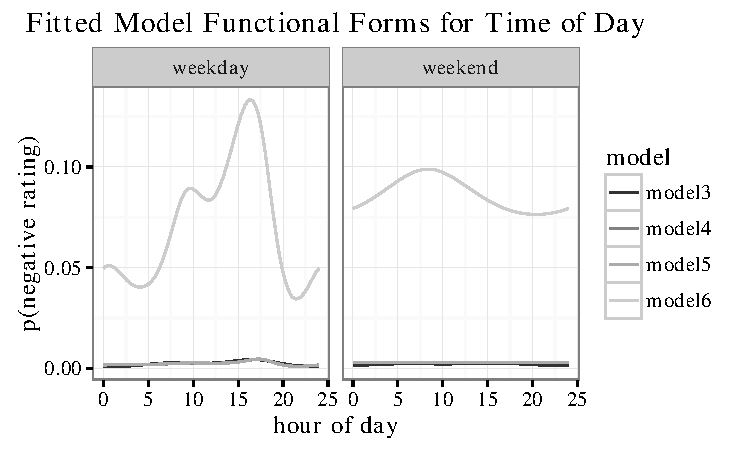
\includegraphics{figure/time_fit_plot.pdf}
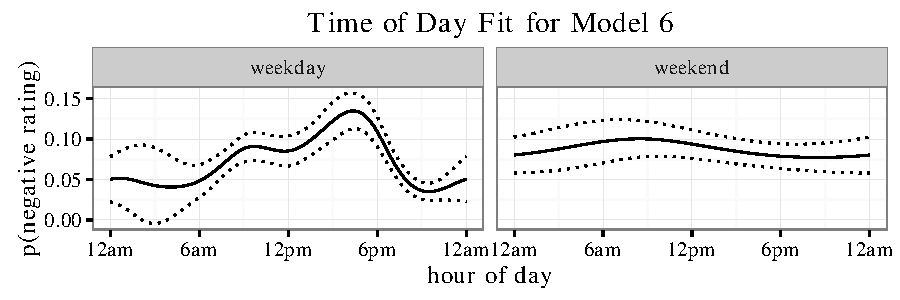
\includegraphics{figure/time_fit_plot_6.pdf}
\caption{Predicted probabilities of a negative rating by time for a typical ride.
The rider was chosen so the intercept was closest to the mean intercept for model
5. The median length and average mean temperature were used, and all other
predictors were set to zero. The dotted lines show $\pm 2$ standard errors from
the predictions.}
\end{figure}

The marginal fits for time of day, shown in
\autoref{fig:model1-time-fit}, are predictable. On weekdays, the
probability of a negative rating peaks in the afternoon from 4--6 p.m.,
around when we expect rush hour traffic, and on weekends it stays steady
throughout the day. While Model 4 and Model 5 give similar fits for time
of day, Model 3's predictions peak at different times on weekdays and
exhibit much more variability on weekends. There are two probable
reasons for these differences: first, the sinusoidal terms are less
flexibile than the splines; second, the splines, because they are
non-parametric functions, penalize complexity of the fit while the
parametric sinusoidal form does not, making the splines more
conservative in their ``curviness.'' The former explains the
discrepancies in the weekday fits while the latter explains the
discrepancies in the weekend fits. Given these differences, fitting time
of day with splines is preferable; there is no motivation to constrain
the functional form to any strict parametric form.

But these marginal time-of-day fits don't just tell a story about our
time terms; they also reveal part of why the random rider intercepts are
such powerful predictors. Notice that in comparing
\autoref{fig:model1-time-fit6} to \autoref{fig:model1-time-fit}, the
scale at which the Model 6 time fitted probabilities vary is much larger
than the scale at which the other models' predictions vary. (The
differences is so large we had to show them in separate plots!) Without
allowing for varying rider intercepts, the time terms take on a
significant role. Yet, interestingly, the time term has nowhere near the
amount of information that the rider intercepts seem to encode,
according to the separation plots in \autoref{tab:modelfits}.

\begin{figure}[tbh]
\centering
\includegraphics[angle = 0,scale = 1]{figure/time_pred_plot.pdf}
\caption[Each of the models predictions for all rides with time of day on the x-axis.
Notice how starting with model 2, daily trends start to emerge. This indicates that the
rider intercepts are picking up on time of day trends, which must be reflected in riders
typical ride.]{\normalsize{Each of the models predictions for all rides with time of day on the x-axis.
Notice how starting with model 2, daily trends start to emerge. This indicates that the
rider intercepts are picking up on time of day trends, which must be reflected in riders
typical ride.}}
\label{fig:time-pred-plot}
\end{figure}

A clearer picture of what is going on is painted in
\autoref{fig:time-pred-plot}. The predictions of Model 1, which has a
fixed intercept and no time dependence, don't vary by time of day. The
models with random intercepts (2--5) show strong temporal patterns, with
concentrated spikes in the morning and evening. Model 6, which had the
time of day spline but a fixed intercept, has a temporal pattern, but
does not represent the same degree time dependence that the random
intercept models do.

One should be cautious about interpreting the intercepts. It's tempting
to say they represent a riders general tendency to rate rides
negatively, but this is ignoring their typical route. Just like how
figure \autoref{fig:time-pred-plot} demonstrates that riders have unique
patterns of what times of days they take rides, riders also likely have
very particular routes that make up the majority of their rides. Because
our models do not take into account the route, the intercepts are likely
encoding the information about a riders typical route.

The fact that riders have apparent patterns of time of ride (and very
likely route of ride), indicates there will be some value in trying to
differentiate the types of riders that are present in this data. Indeed,
one way of looking at the range of probabilities of giving a negative
rating different riders have (demonstrated in figure
\autoref{fig:rider-pred}) is that some are more likely to offer useful
information. In the next chapter, we will attempt to pick apart
different groups of riders, and attempt to characterize their patterns
of when and how long they ride.

\end{document}
